% Desain split data. Gaya visual mengikuti architecture-paddle.tex.
% Kompilasi: pdflatex architecture-split.tex
\documentclass[border=14pt,tikz]{standalone}
\usepackage[T1]{fontenc}
\usepackage{tikz}
\usetikzlibrary{arrows.meta,positioning,fit,backgrounds,calc}
\pgfdeclarelayer{bgA}\pgfdeclarelayer{bgB}
\pgfsetlayers{bgB,bgA,main}

\definecolor{gGray}  {HTML}{E8EAED}
\definecolor{gBlueBg}{HTML}{DCEAFB}\definecolor{gBlue}  {HTML}{2E6DB4}
\definecolor{gPurBg} {HTML}{EFE4F7}\definecolor{gPur}   {HTML}{6B3FA0}
\definecolor{gPinkBg}{HTML}{FBE0E8}\definecolor{gPink}  {HTML}{B03A5B}
\definecolor{gGreen} {HTML}{2E8B57}
\definecolor{gCream} {HTML}{FBF3DE}\definecolor{gTan}   {HTML}{A8871F}
\definecolor{gAmber} {HTML}{E8873C}
\definecolor{gEdge}  {HTML}{5F6368}
\definecolor{gMuted} {HTML}{80868B}

\begin{document}\sffamily
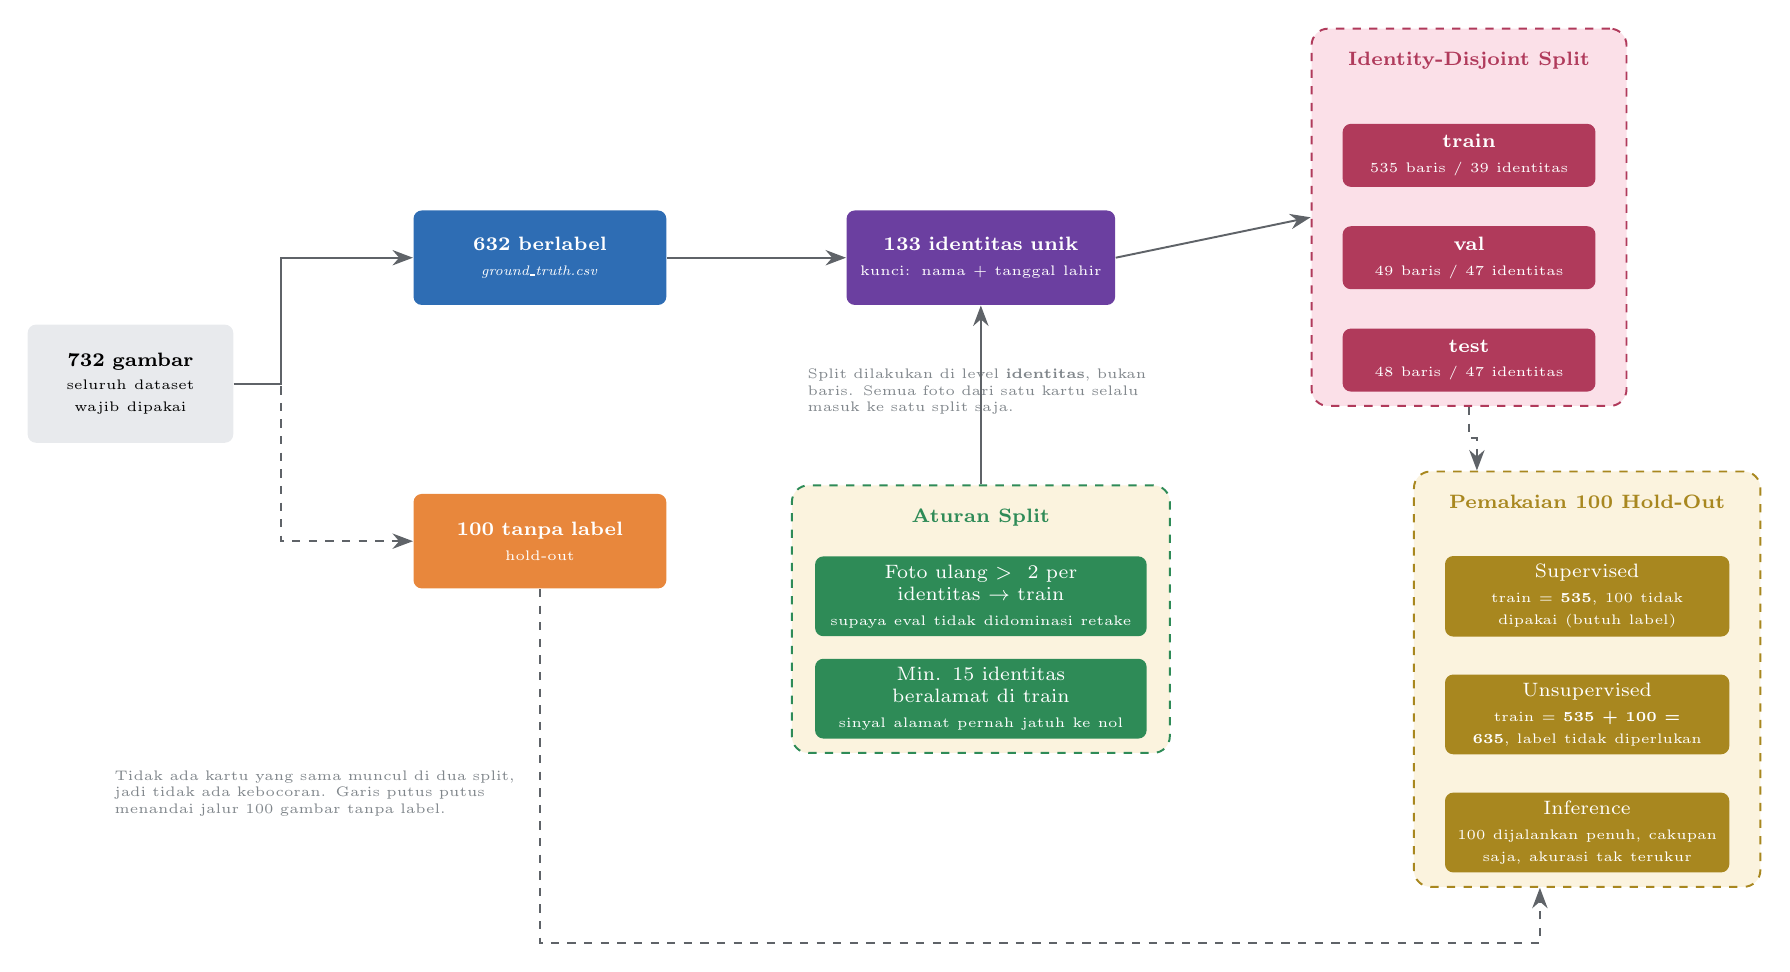
\begin{tikzpicture}[
  x=1mm, y=1mm, font=\scriptsize,
  blk/.style={rounded corners=3pt, draw=none, align=center, text=white,
              inner sep=3pt, minimum height=8mm, text width=26mm},
  grp/.style={rounded corners=6pt, dashed, line width=0.7pt, inner sep=5pt},
  lbl/.style={font=\scriptsize\bfseries, align=center},
  ar/.style={-{Stealth[length=2.6mm]}, draw=gEdge, line width=0.7pt},
  ard/.style={ar, dashed},
]

% ---------------------------------------------------------------- sumber
\node[blk, fill=gGray, text=black, text width=24mm, minimum height=15mm] at (0,0) (all)
  {\textbf{732 gambar}\\[2pt]{\tiny seluruh dataset\\wajib dipakai}};

% ---------------------------------------------------------------- dua cabang
\node[blk, fill=gBlue, text width=30mm, minimum height=12mm] at (52,16) (lab)
  {\textbf{632 berlabel}\\[1pt]{\tiny \textit{ground\_truth.csv}}};
\node[blk, fill=gAmber, text width=30mm, minimum height=12mm] at (52,-20) (unlab)
  {\textbf{100 tanpa label}\\[1pt]{\tiny hold-out}};

% ---------------------------------------------------------------- identitas
\node[blk, fill=gPur, text width=32mm, minimum height=12mm] at (108,16) (idg)
  {\textbf{133 identitas unik}\\[1pt]{\tiny kunci: nama + tanggal lahir}};

\node[align=left, text=gMuted, font=\tiny, text width=44mm] at (108,-1)
  {Split dilakukan di level \textbf{identitas}, bukan baris.
   Semua foto dari satu kartu selalu masuk ke satu split saja.};

% ---------------------------------------------------------------- tiga split
\node[blk, fill=gPink, text width=30mm] at (170,29) (tr)
  {\textbf{train}\\[1pt]{\tiny 535 baris / 39 identitas}};
\node[blk, fill=gPink, text width=30mm] at (170,16) (va)
  {\textbf{val}\\[1pt]{\tiny 49 baris / 47 identitas}};
\node[blk, fill=gPink, text width=30mm] at (170,3) (te)
  {\textbf{test}\\[1pt]{\tiny 48 baris / 47 identitas}};
\node[lbl, text=gPink, text width=34mm] at (170,41) (spl) {Identity-Disjoint Split};
\begin{pgfonlayer}{bgB}
  \node[grp, draw=gPink, fill=gPinkBg, fit=(spl)(tr)(va)(te)] (gS) {};
\end{pgfonlayer}

% ---------------------------------------------------------------- aturan
\node[blk, fill=gGreen, text width=40mm, minimum height=9mm] at (108,-27) (r1)
  {Foto ulang $>2$ per identitas $\rightarrow$ train\\[1pt]{\tiny supaya eval tidak didominasi retake}};
\node[blk, fill=gGreen, text width=40mm, minimum height=9mm] at (108,-40) (r2)
  {Min. 15 identitas beralamat di train\\[1pt]{\tiny sinyal alamat pernah jatuh ke nol}};
\node[lbl, text=gGreen, text width=42mm] at (108,-17) (rl) {Aturan Split};
\begin{pgfonlayer}{bgB}
  \node[grp, draw=gGreen, fill=gCream, fit=(rl)(r1)(r2)] (gR) {};
\end{pgfonlayer}

% ---------------------------------------------------------------- pemakaian 100
\node[blk, fill=gTan, text width=34mm, minimum height=10mm] at (185,-27) (u1)
  {Supervised\\[1pt]{\tiny train = \textbf{535}, 100 tidak dipakai (butuh label)}};
\node[blk, fill=gTan, text width=34mm, minimum height=10mm] at (185,-42) (u2)
  {Unsupervised\\[1pt]{\tiny train = \textbf{535 + 100 = 635}, label tidak diperlukan}};
\node[blk, fill=gTan, text width=34mm, minimum height=10mm] at (185,-57) (u3)
  {Inference\\[1pt]{\tiny 100 dijalankan penuh, cakupan saja, akurasi tak terukur}};
\node[lbl, text=gTan, text width=38mm] at (185,-15) (ul) {Pemakaian 100 Hold-Out};
\begin{pgfonlayer}{bgB}
  \node[grp, draw=gTan, fill=gCream, fit=(ul)(u1)(u2)(u3)] (gU) {};
\end{pgfonlayer}

% ---------------------------------------------------------------- panah
\draw[ar]  (all.east) -- ++(6,0) |- (lab.west);
\draw[ard] (all.east) -- ++(6,0) |- (unlab.west);
\draw[ar]  (lab.east) -- (idg.west);
\draw[ar]  (idg.east) -- (gS.west);
\draw[ar]  (gR.north) -- ++(0,3) -| (idg.south);
\draw[ard] (unlab.south) -- ++(0,-45) -| ([xshift=-6mm]gU.south);
\draw[ard] (gS.south) -- ++(0,-4) -| ([xshift=-14mm]gU.north);

% catatan
\node[align=left, text=gMuted, font=\tiny, text width=52mm] at (24,-52)
  {Tidak ada kartu yang sama muncul di dua split, jadi tidak ada kebocoran.
   Garis putus putus menandai jalur 100 gambar tanpa label.};

\end{tikzpicture}
\end{document}
